\documentclass[11pt,a4paper]{article}
\usepackage[T1]{fontenc}
\usepackage[margin=2.3cm]{geometry}
\usepackage{amsmath,amssymb}
\usepackage{graphicx}
\usepackage[dvipsnames]{xcolor}
\usepackage{enumitem}
\usepackage[colorlinks=true,linkcolor=blue,urlcolor=blue]{hyperref}
\setlength{\parskip}{0.6em}
\setlength{\parindent}{0pt}
\begin{document}

\begin{center}{\LARGE\bfseries openmechanism}\\[0.4em]{\large Tune a kinetic mechanism until its simulations match experiments, in three sessions.}\\[0.2em]\small PAN IIT OSS explainer \textbullet{} secondary school to diploma / undergraduate (levels 3-5)\end{center}

\section*{Why this exists}
A chemical mechanism is a list of reactions whose rate constants come from experiments and theory, each with an uncertainty. This explainer shows, with invented numbers, how a mechanism is tuned against experimental data, how to say how well each rate constant is known, and what an experiment can and cannot tell you.

\section*{The end goal}
Optimise a kinetic mechanism against experiments. The end goal is optimising a kinetic mechanism against experiments: matching simulations to measurements while keeping every rate constant honest about its uncertainty. The same ideas apply to any model with parameters fitted to data.

\section*{How the three sessions build up}
\begin{enumerate}[nosep]
\item \textbf{Session 1: A reaction network as equations, and what an experiment sees} (Level 1, conceptual interactive model, 60 min).
\item \textbf{Session 2: Arrhenius, the 1000/T plot, and which rate an experiment feels} (Level 2, mathematical engineering model, 75 min).
\item \textbf{Session 3: Calibrating a toy mechanism against noisy experiments} (Level 3, simulation and validation, 90 min).
\end{enumerate}

\section{Session 1: A reaction network as equations, and what an experiment sees}

\subsection*{A. Real-world problem}
Burning a fuel is never one step: molecules turn into other molecules, which turn into others. A list of such steps, each with a speed, is called a mechanism, and real ones have hundreds of steps. An experiment cannot watch every molecule; it measures one thing, such as how much of an intermediate is present at a few moments. Can we build the smallest possible mechanism, two steps, write it as equations, and see what a measurement of the middle molecule B can reveal about the two speeds? (Toy numbers throughout; this is a teaching model, not real chemistry data.)

\subsection*{B. Concept and theory}
A rate constant k tells how fast a reaction proceeds: in A -\textgreater{} B the amount of A drops at the speed k1 times the amount of A. For A -\textgreater{} B -\textgreater{} C we get three linked equations: A only decays, B is fed by A and drained into C, and C only grows. The total A + B + C stays constant because molecules are not lost. For k1 different from k2 the exact solution is a difference of two exponentials. B starts at zero, rises while A is plentiful, and falls once it drains faster than it is fed; it peaks exactly when the feed k1 A equals the drain k2 B. Euler's method replaces the smooth change by small jumps of size (rate x time step), and gets better as the step shrinks. An experiment gives noisy numbers at a few times, so many pairs (k1, k2) can look nearly right; the misfit (root-mean-square difference) tells how far a model is from the data.

\begin{itemize}[nosep]
\item A, B, C: concentrations of the three molecules (mol/L (toy))
\item t: time (s)
\item k1, k2: rate constants of A -\textgreater{} B and B -\textgreater{} C (1/s)
\item dt: Euler time step (s)
\item t*: time at which B is largest (s)
\end{itemize}

\begin{equation*}
\frac{dA}{dt}=-k_1A,\qquad \frac{dB}{dt}=k_1A-k_2B,\qquad \frac{dC}{dt}=k_2B
\end{equation*}

\begin{equation*}
A(t)=e^{-k_1t},\qquad B(t)=\frac{k_1}{k_2-k_1}\left(e^{-k_1t}-e^{-k_2t}\right),\qquad C=1-A-B
\end{equation*}

\begin{equation*}
t^{*}=\frac{\ln(k_2/k_1)}{k_2-k_1},\qquad B_{\max}=\left(\frac{k_1}{k_2}\right)^{k_2/(k_2-k_1)}
\end{equation*}

\begin{equation*}
y_{n+1}=y_n+\Delta t\,f(y_n)\quad\text{(Euler step)}
\end{equation*}

\begin{center}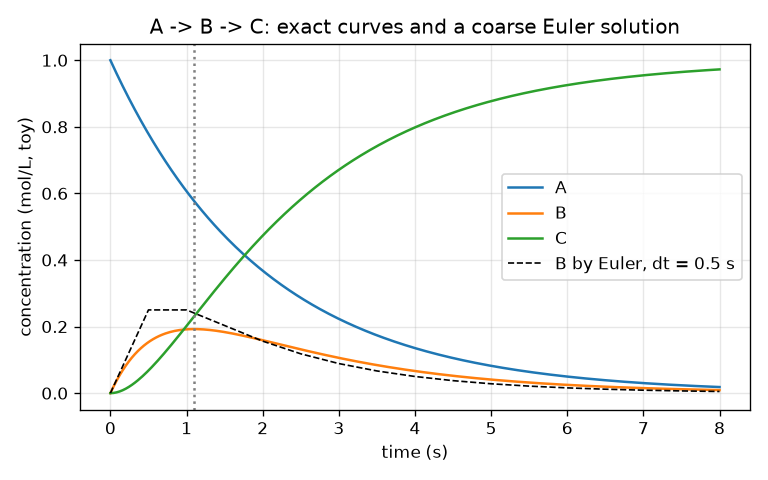
\includegraphics[width=0.85\linewidth]{figures/s01_abc_curves.png}\\\small A, B and C against time for k1 = 0.5 and k2 = 1.5 per s, with a coarse Euler solution (dashed).\end{center}

\subsection*{E. Worked example}
With k1 = 0.5 per s and k2 = 1.5 per s, when does B peak, how large is B then, and what is B at t = 1 s?
\begin{enumerate}[nosep]
\item Peak time: t* = ln(k2/k1) / (k2 - k1) = ln 3 / 1.0 = 1.0986 s.
\item Peak height: B = (k1/k2)\textasciicircum{}(k2/(k2-k1)) = (1/3)\textasciicircum{}1.5 = 0.1925 mol/L.
\item Check at the peak: A = exp(-0.5 x 1.0986) = 0.577, so feed k1 A = 0.289 and drain k2 B = 1.5 x 0.1925 = 0.289. They are equal, as they must be at a maximum.
\item At t = 1 s: B = 0.5 / 1.0 x (exp(-0.5) - exp(-1.5)) = 0.5 x (0.6065 - 0.2231) = 0.1917 mol/L, just below the peak, as expected.
\end{enumerate}
\textbf{Answer.} B peaks at 1.099 s with 0.1925 mol/L; at 1 s it is 0.1917 mol/L.

\subsection*{F. Questions}
\begin{enumerate}[nosep]
\item \textbf{Conceptual.} Why does B rise first and then fall, even though both reactions run all the time? At which moment is its rate of change zero?
\item \textbf{Numerical.} For k1 = 0.4 per s and k2 = 0.8 per s, find the time and height of the peak of B. Check the units and that the answer is sensible.
\item \textbf{Graph and simulation interpretation.} In the concentration graph with k1 = 0.5 and k2 = 1.5, which curve rises fastest at the moment B is at its peak, and why?
\item \textbf{Design and optimisation challenge.} Design: you may measure B at one time only. The unknown mechanism is either (k1, k2) = (0.5, 1.5) or (1.5, 0.5), and the measurement noise is 0.01 mol/L. Which time do you choose, and how well will you tell the two apart?
\end{enumerate}

\section{Session 2: Arrhenius, the 1000/T plot, and which rate an experiment feels}

\subsection*{A. Real-world problem}
Hot gas reacts much faster than cold gas: raising the temperature from 1000 K to 1200 K can speed a reaction up fivefold. A mechanism therefore stores a formula for every rate constant, and calibration adjusts that formula. But which of the hundreds of rate constants does a given experiment actually care about? If we nudge one by 1 percent, how much does the measured ignition delay move? And if we can afford only two experiments, at which temperatures should we run them? (Toy numbers; not data for any real fuel.)

\subsection*{B. Concept and theory}
The modified Arrhenius form says k(T) = A T\textasciicircum{}n exp(-Ea / R T). The exponential is the fraction of molecular encounters that carry at least the activation energy Ea; R = 8.314 J/(mol K) converts temperature into energy per mole. Taking logarithms gives ln k = ln A + n ln T - Ea / (R T), a straight line in 1/T when n = 0; plotting against 1000/T keeps the numbers near 1, and the slope is -Ea/(1000 R) per unit of 1000/T, so a line fitted through measured rate constants gives Ea. For the toy ignition delay we use a branching chain F -\textgreater{} R (k1), F + R -\textgreater{} 2 R (k2), R -\textgreater{} P (k3). While fuel is plentiful the radical R grows at the rate g = k2 F0 - k3 and is seeded by k1, so the radical amount reaches F0/2 after tau = ln(1 + g / (2 k1)) / g (an approximation that ignores fuel use). The sensitivity S\_i = d ln tau / d ln k\_i is the percent change of tau per percent change of k\_i; we compute it by a central difference and verify it against the derivative. Each experiment adds a row of sensitivities to a matrix J; with noise sigma, the uncertainty of the scale factors of the rate constants is the square root of the diagonal of (J\textasciicircum{}T J)\textasciicircum{}-1.

\begin{itemize}[nosep]
\item k: rate constant (1/s (first order))
\item A: pre-exponential factor, carries the unit of k (1/s (for n = 0))
\item n: temperature exponent (no unit)
\item Ea: activation energy (J/mol (kJ/mol in the app))
\item R: gas constant, 8.314 J/(mol K) (J/(mol K))
\item T: absolute temperature (K)
\item tau: ignition delay (s)
\item S\_i: sensitivity d ln tau / d ln k\_i (no unit)
\item sigma: noise in ln tau (0.05 = 5 percent) (no unit)
\end{itemize}

\begin{equation*}
k(T)=A\,T^{n}\exp\!\left(-\frac{E_a}{R\,T}\right)
\end{equation*}

\begin{equation*}
\ln k=\ln A+n\ln T-\frac{E_a}{R}\cdot\frac{1}{T},\qquad \text{slope on a }\frac{1000}{T}\text{ plot}=-\frac{E_a}{1000\,R}
\end{equation*}

\begin{equation*}
g=k_2F_0-k_3,\qquad \tau=\frac{1}{g}\ln\!\left(1+\frac{g}{2k_1}\right)
\end{equation*}

\begin{equation*}
S_i=\frac{\partial\ln\tau}{\partial\ln k_i}\approx\frac{\ln\tau(k_ie^{\varepsilon})-\ln\tau(k_ie^{-\varepsilon})}{2\varepsilon}
\end{equation*}

\begin{equation*}
\mathrm{Cov}=(J^{\mathsf T}J)^{-1},\qquad J_{ij}=\frac{S_{ij}}{\sigma}
\end{equation*}

\begin{center}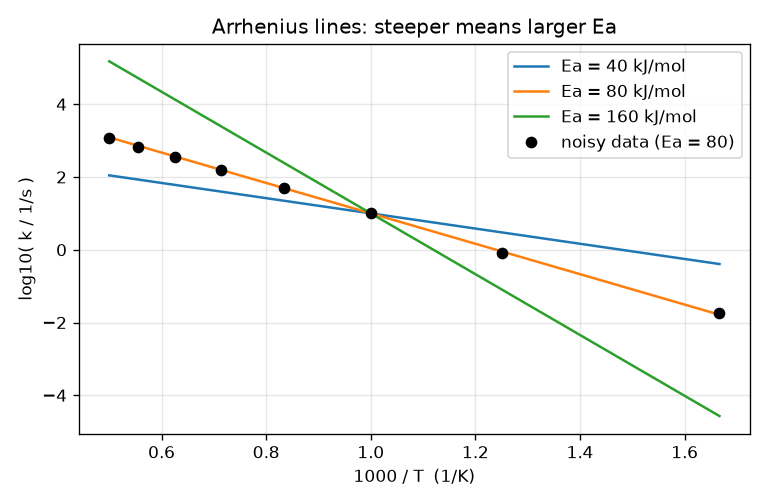
\includegraphics[width=0.85\linewidth]{figures/s02_arrhenius_1000T.png}\\\small Arrhenius lines on the 1000/T plot: steeper means larger activation energy.\end{center}

\subsection*{E. Worked example}
A reaction has Ea = 80 kJ/mol and n = 0. By what factor does k increase from 1000 K to 1200 K? Then find the toy ignition delay at 1000 K from the formula.
\begin{enumerate}[nosep]
\item Ratio = exp(Ea / R x (1/1000 - 1/1200)) = exp(80000 / 8.3145 x 1.6667e-4).
\item 80000 / 8.3145 = 9621.8; times 1.6667e-4 = 1.6036; exp(1.6036) = 4.97. Units: Ea / (R T) is dimensionless, so the ratio is a pure number.
\item Toy ignition delay at 1000 K: k1 = 0.002 per s, k2 = 30 L/(mol s), k3 = 10 per s, F0 = 1 mol/L, so g = 30 x 1 - 10 = 20 per s.
\item tau = ln(1 + 20 / (2 x 0.002)) / 20 = ln(5001) / 20 = 8.517 / 20 = 0.4259 s.
\end{enumerate}
\textbf{Answer.} The rate constant grows by a factor of 4.97, and the toy ignition delay at 1000 K is 0.4259 s.

\subsection*{F. Questions}
\begin{enumerate}[nosep]
\item \textbf{Conceptual.} Why is a plot of log k against 1000/T a straight line for the simple Arrhenius form, and what physical quantity does its slope give?
\item \textbf{Numerical.} A reaction has Ea = 120 kJ/mol (n = 0). Find the factor by which k grows from 1000 K to 1100 K, and the slope of ln k against 1000/T.
\item \textbf{Graph and simulation interpretation.} Look at the sensitivity graph. Which rate constant does the ignition delay feel most at 900 K, and at 1400 K? What does a negative or a positive sign mean?
\item \textbf{Design and optimisation challenge.} Design: you can run two experiments at two of the temperatures 900, 1000, 1100, 1200, 1300, 1400 K (5 percent noise) to learn the scale factors of k1 and k2. Which pair do you choose, which pair is worst, and why?
\end{enumerate}

\section{Session 3: Calibrating a toy mechanism against noisy experiments}

\subsection*{A. Real-world problem}
A kinetic mechanism has rate constants that nobody knows exactly. Experiments, here ignition delays at several temperatures, measure what the mechanism should predict. Calibration moves the rate constants until the simulations match, and it must also say how well the data pinned each one down. Can we write the solver, generate fake experiments from a known truth, recover that truth by least squares, and see honestly which parameters the data cannot determine? (Everything is a toy: four invented reactions and invented numbers, far simpler than real combustion chemistry, and not usable for engineering decisions.)

\subsection*{B. Concept and theory}
The toy mechanism is F -\textgreater{} R (k1), F + R -\textgreater{} 2R (k2), R -\textgreater{} P (k3), F -\textgreater{} P (k4), solved as two coupled ODEs for fuel F and radical R. Rates differ by large factors, which makes real mechanisms stiff: explicit methods need tiny steps. We use the trapezoidal rule, which solves for the new state at each step with Newton's method, is second-order accurate and stays bounded for large steps. Ignition delay tau is the time when F reaches F0/2. We calibrate theta = (ln s1, ln s2), the logarithms of scale factors multiplying k1 and k2 at all temperatures. For each experiment the residual is r\_i = (ln tau\_model - ln tau\_observed) / sigma\_i. Levenberg-Marquardt steps by delta = -(J\textasciicircum{}T J + lambda D)\textasciicircum{}-1 J\textasciicircum{}T r with J the Jacobian of the residuals (by finite differences). At the optimum the covariance of the estimates is (J\textasciicircum{}T J)\textasciicircum{}-1, which gives one-sigma uncertainties and an ellipse; the reduced chi-square sum(r\textasciicircum{}2)/(n - 2) should be near 1. With several datasets, the power-mean objective M\_p = (mean over datasets of E\_d\textasciicircum{}p)\textasciicircum{}(1/p) with E\_d the root-mean-square residual of dataset d is minimised by re-weighting each dataset by E\_d\textasciicircum{}(p-2)/n\_d: p = 2 gives every dataset the same total weight however many points it has. Because the data are synthetic, we can compare the answer with the truth, which is impossible for real experiments.

\begin{itemize}[nosep]
\item F, R, P: fuel, radical, product concentrations (mol/L (toy))
\item k1..k4: rate constants (k2 in L/(mol s), others in 1/s) (see text)
\item s: scale factor on a rate constant (1 = nominal) (no unit)
\item theta: parameters (ln s1, ln s2) (no unit)
\item tau: ignition delay: F = F0/2 (s)
\item sigma: noise in ln tau (0.05) (no unit)
\item r: residual in units of noise widths (no unit)
\item J: Jacobian of the residuals (per unit of theta)
\item Cov: covariance of the estimated theta (no unit)
\end{itemize}

\begin{equation*}
\frac{dF}{dt}=-(k_1+k_4)F-k_2FR,\qquad \frac{dR}{dt}=k_1F+k_2FR-k_3R
\end{equation*}

\begin{equation*}
y_{n+1}=y_n+\tfrac{\Delta t}{2}\big(f(y_n)+f(y_{n+1})\big)\quad\text{(trapezoidal rule, solved by Newton)}
\end{equation*}

\begin{equation*}
r_i=\frac{\ln\tau_i^{\mathrm{model}}(\theta)-\ln\tau_i^{\mathrm{obs}}}{\sigma_i},\qquad \theta=(\ln s_1,\ln s_2)
\end{equation*}

\begin{equation*}
\delta=-\big(J^{\mathsf T}J+\lambda D\big)^{-1}J^{\mathsf T}r,\qquad \mathrm{Cov}=(J^{\mathsf T}J)^{-1}
\end{equation*}

\begin{equation*}
M_p=\Big(\tfrac1D\sum_{d}E_d^{\,p}\Big)^{1/p},\qquad E_d=\sqrt{\tfrac1{n_d}\sum_{i\in d}r_i^2}
\end{equation*}

\begin{center}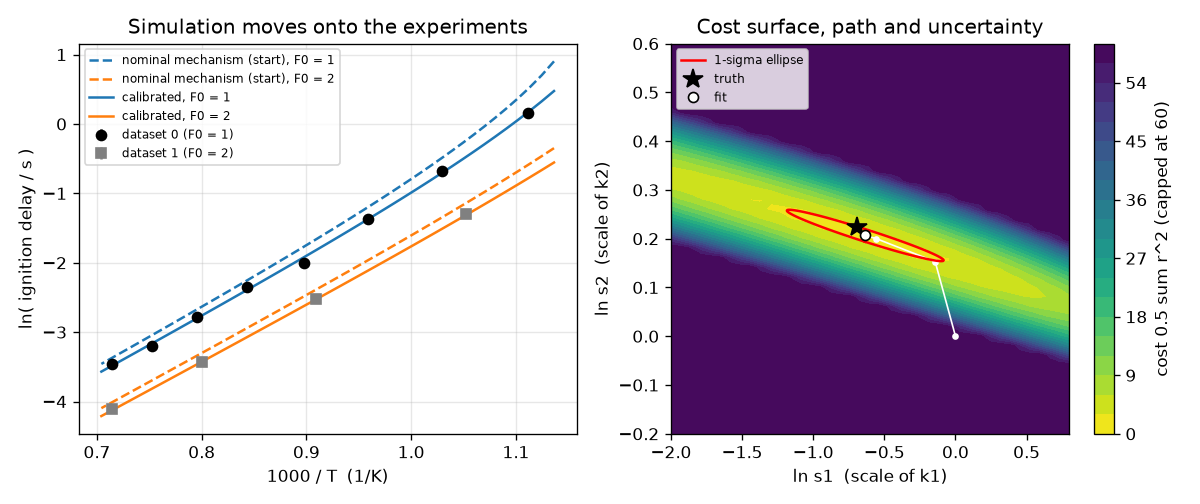
\includegraphics[width=0.85\linewidth]{figures/s03_calibration.png}\\\small Left: data, nominal (dashed) and calibrated (solid) curves. Right: cost surface, fit path, one-sigma ellipse and truth.\end{center}

\subsection*{E. Worked example}
Calibrate from the nominal mechanism (s1 = s2 = 1) using the synthetic data set with seed 1 (truth: s1 = 0.5, s2 = 1.25). Report the fit, its uncertainty, and whether the truth is recovered.
\begin{enumerate}[nosep]
\item Start: theta = (0, 0), cost 0.5 sum r\textasciicircum{}2 = 72.5. Levenberg-Marquardt reaches theta = (-0.634, 0.207) in about 5 iterations with cost 2.02.
\item Scale factors: s1 = exp(-0.634) = 0.53 and s2 = exp(0.207) = 1.23, compared with the truth 0.50 and 1.25.
\item Uncertainty from (J\textasciicircum{}T J)\textasciicircum{}-1: one-sigma of (ln s1, ln s2) = (0.55, 0.053), correlation -0.97. So k2 is known to about 5 percent and k1 only to a factor of about e\textasciicircum{}0.55 = 1.7.
\item z-scores = (fit - truth) / sigma: (-0.634 + 0.693) / 0.551 = 0.11 and (0.207 - 0.223) / 0.053 = -0.3. Both are well inside 2 sigma, so the truth is recovered within its uncertainty. The reduced chi-square is 0.40 with 10 degrees of freedom, consistent with noise-only residuals for one noise draw.
\end{enumerate}
\textbf{Answer.} The fit gives s1 = 0.53 and s2 = 1.23 (truth 0.50 and 1.25); the truth lies within 0.11 and 0.3 standard deviations; k2 is well determined (5 percent), k1 is not (a factor of 1.7).

\subsection*{F. Questions}
\begin{enumerate}[nosep]
\item \textbf{Conceptual.} The fitted ln s1 has a one-sigma uncertainty of 0.55 while ln s2 has 0.053. Explain why the data pin k2 down much better, and why the two uncertainties are strongly correlated.
\item \textbf{Numerical.} The calibration used 12 experiments and gave a one-sigma uncertainty of 0.053 for ln s2. If you repeat the whole campaign 4 times (48 experiments, same noise), what uncertainty do you expect? What would 4 times less noise give?
\item \textbf{Graph and simulation interpretation.} In the cost-surface picture, what does the long axis of the valley tell you, and where would the one-sigma ellipse of a set of experiments at 1300 and 1400 K only look different?
\item \textbf{Design and optimisation challenge.} Design: you have 12 experiments to spend, all with 1 mol/L fuel, and the temperature may be 900 to 1400 K. Compare the shipped design (8 temperatures plus 4 at 2 mol/L) with putting 6 experiments at 900 K and 6 at 1400 K. Which gives the smaller uncertainty of ln s1, and what could go wrong?
\end{enumerate}

\section{Real-world mini-project}
\textbf{Calibrate two rate constants from a synthetic ignition-delay data set.} A lab hands you 12 noisy ignition delays (\texttt{make\_dataset(seed=42)} from Session 3: 8 temperatures at 1 mol/L fuel and 4 at 2 mol/L, 5 percent noise). The nominal mechanism is wrong: the scale factors of k1 and k2 are unknown. Use \texttt{calibrate} from Session 3 to find them, then use \texttt{covariance} to report how well each is known and draw the one-sigma ellipse. Because the data are synthetic you may then compare with \texttt{TRUTH}, which a real lab never could.

\section{The path ahead}
\begin{enumerate}[nosep]
\item \textbf{Session 4: Choose experiments well.} A small design tool that, for a budget of 12 experiments, picks conditions that minimise the one-sigma uncertainty of both scale factors.
\item \textbf{Session 5: Fit an activation energy too.} A calibration with a parameter that shifts Ea of k2, plus its uncertainty.
\item \textbf{Session 6: Survive a biased dataset.} A calibration in which one dataset carries an unknown offset, handled by an extra fitted offset or a robust objective.
\item \textbf{Session 7: Propagate the uncertainty into predictions.} Sampling parameter sets from the ellipse and simulating the ignition delay at a new temperature.
\item \textbf{Session 8: Reproduce the Target.} An animation of the curves converging onto the data while the ellipse shrinks.
\end{enumerate}

\section{Answers and hints}

\subsection*{Session 1}
\begin{enumerate}[nosep]
\item \textbf{Conceptual.} Hint: Compare how fast B is fed with how fast it drains. Solution: B is fed at k1 A, which is large at the start (A is plentiful) and shrinks as A is used up; B is drained at k2 B, which is zero at the start and grows with B. Early on the feed wins and B rises; later the drain wins and B falls. The rate of change of B is zero exactly when feed equals drain, k1 A = k2 B, which is the peak.
\item \textbf{Numerical.} Hint: Use t* = ln(k2/k1)/(k2 - k1) and B\_max = (k1/k2)\textasciicircum{}(k2/(k2-k1)). Solution: t* = ln 2 / 0.4 = 0.6931 / 0.4 = 1.733 s. B\_max = (0.5)\textasciicircum{}(0.8/0.4) = 0.5\textasciicircum{}2 = 0.25 mol/L. Units: ln of a ratio has no unit, divided by 1/s gives s; B is a fraction of the starting 1 mol/L, so 0.25 mol/L is plausible (less than 1). Check with the full formula: B(1.733) = 0.4/0.4 x (exp(-0.693) - exp(-1.386)) = 0.5 - 0.25 = 0.25.
\item \textbf{Graph and simulation interpretation.} Hint: C grows at the speed k2 B. Solution: C grows at k2 B. B is largest at its peak, so the growth rate of C is largest there: the C curve is steepest at 1.1 s. The A curve is falling all the time and is steepest at t = 0.
\item \textbf{Design and optimisation challenge.} Hint: Compute B(t) for both and look at the difference. A useful fact: swapping k1 and k2 changes B by a constant factor. Solution: Swapping the two rate constants multiplies B by k2/k1 = 3 at every time, so the second mechanism always gives 3 times as much B. The difference is largest where B is largest, at the common peak time 1.099 s: 0.1925 against 0.577 mol/L, a difference of 0.385 mol/L, about 38 times the noise. Any time works in principle, but the peak gives the largest margin. Trade-off: a measurement at t = 0 (B = 0) tells nothing, and very late times give tiny signals close to the noise.
\end{enumerate}

\subsection*{Session 2}
\begin{enumerate}[nosep]
\item \textbf{Conceptual.} Hint: Take the logarithm of k = A exp(-Ea / R T) and compare with y = c + m x. Solution: ln k = ln A - (Ea / R) (1/T) has the form c + m x with x = 1/T, so it is a straight line. The slope is -Ea/R per unit of 1/T, or -Ea/(1000 R) per unit of 1000/T. A steeper line therefore means a larger activation energy: a reaction that is more sensitive to temperature.
\item \textbf{Numerical.} Hint: Ratio = exp(Ea/R x (1/1000 - 1/1100)). Slope = -Ea/(1000 R). Solution: Ea/R = 120000 / 8.3145 = 14433 K. (1/1000 - 1/1100) = 9.091e-5 per K. Product = 1.312, exp(1.312) = 3.71. The slope is -14433 / 1000 = -14.43 per unit of 1000/T (in log10: -6.27). Sanity check: a larger Ea than the worked example (80) with a smaller temperature range (100 K instead of 200 K) gives a similar order, 3.7 versus 5.0.
\item \textbf{Graph and simulation interpretation.} Hint: Compare the absolute values of the three curves at each temperature. Solution: At 900 K the magnitudes are about 2.06 (k2), 1.17 (k3) and 0.11 (k1): k2 dominates, k3 is also important. At 1400 K they are 0.93 (k2), 0.08 (k3) and 0.15 (k1): k2 again dominates, k3 is nearly irrelevant. A negative sign (k1, k2) means a faster reaction shortens the delay; the positive sign of k3 means a faster radical loss lengthens it.
\item \textbf{Design and optimisation challenge.} Hint: Use \texttt{design\_std(pair)} for all 15 pairs and compare the first column (ln s1) and second column (ln s2). Solution: The widest pair, 900 and 1400 K, is best: one-sigma uncertainties of (ln s1, ln s2) = (0.57, 0.047). The two hottest, 1300 and 1400 K, are worst: (5.5, 0.83): the sensitivity rows are almost parallel, so the two unknowns cannot be separated. Reason: k1 and k2 have different activation energies, so their effects differ most when the temperatures are far apart. Trade-offs: the coldest experiment is slowest and may be hard to run; and the toy formula ignores the fuel being used up, so check a candidate design with the full solver of Session 3 before relying on it.
\end{enumerate}

\subsection*{Session 3}
\begin{enumerate}[nosep]
\item \textbf{Conceptual.} Hint: Remember the sensitivities of Session 2: tau depends on k1 only through a logarithm. Solution: The ignition delay is tau = ln(1 + g/(2 k1)) / g approximately: it depends on k1 only inside a logarithm (sensitivity about -0.1), but on k2 almost proportionally (sensitivity about -1 to -2). A 5 percent measurement therefore fixes k2 to about 5 percent but k1 only to a large factor. A change of k1 can be partly undone by a small change of k2 (they act on the delay in the same direction through the same quantity g), so the cost surface has a tilted narrow valley and the estimates are anti-correlated (about -0.97).
\item \textbf{Numerical.} Hint: Cov = (J\textasciicircum{}T J)\textasciicircum{}-1, and J\textasciicircum{}T J adds up over experiments. Solution: Four repeats of every row multiply J\textasciicircum{}T J by 4, so the covariance is divided by 4 and the standard deviation by 2: 0.053 / 2 = 0.027 (a 2.7 percent uncertainty in k2). With 4 times less noise, J is multiplied by 4 so J\textasciicircum{}T J by 16 and the standard deviation drops by 4: 0.013. Sanity check: the uncertainty scales linearly with sigma and as one over the square root of the number of equal experiments (the lesson checks the halving numerically). This assumes independent noise and a model that is linear near the optimum.
\item \textbf{Graph and simulation interpretation.} Hint: Think of how a parameter combination that does not change the cost relates to the uncertainty. Solution: The long axis is the combination of parameters the data hardly constrain: moving along it changes the cost very little. The ellipse is the contour where the cost rises by a fixed amount, so it is long along that axis. Experiments at similar temperatures give almost parallel Jacobian rows (Session 2), so the valley becomes even longer and thinner: the ellipse stretches further and in the limit becomes a line.
\item \textbf{Design and optimisation challenge.} Hint: Build a data set dictionary like \texttt{make\_dataset} produces and call \texttt{covariance(TRUTH, data)}. Solution: Shipped design: one-sigma of ln s1 about 0.57 at the truth. 6 experiments each at 900 and 1400 K: 0.35. Widely separated temperatures give very different sensitivity rows and pin both parameters better. Risks: (i) the coldest experiment must really be run, and at 900 K with only 0.5 mol/L fuel the toy mechanism does not ignite at all, so conditions must be checked with the solver first; (ii) putting all experiments at two temperatures leaves no way to detect that the model is wrong between them; (iii) the covariance is a linear estimate. A design with a few points in the middle trades some uncertainty for robustness.
\end{enumerate}

\section{How to join}
Read \texttt{CONTRIBUTING.md} in the repository, then pick an issue labelled \texttt{good first issue}. Repository: \url{https://github.com/KrunalPanchal1995/openmechanism}

\end{document}
